% Options for packages loaded elsewhere
\PassOptionsToPackage{unicode}{hyperref}
\PassOptionsToPackage{hyphens}{url}
%
\documentclass[
]{article}
\usepackage{amsmath,amssymb}
\usepackage{lmodern}
\usepackage{iftex}
\ifPDFTeX
  \usepackage[T1]{fontenc}
  \usepackage[utf8]{inputenc}
  \usepackage{textcomp} % provide euro and other symbols
\else % if luatex or xetex
  \usepackage{unicode-math}
  \defaultfontfeatures{Scale=MatchLowercase}
  \defaultfontfeatures[\rmfamily]{Ligatures=TeX,Scale=1}
\fi
% Use upquote if available, for straight quotes in verbatim environments
\IfFileExists{upquote.sty}{\usepackage{upquote}}{}
\IfFileExists{microtype.sty}{% use microtype if available
  \usepackage[]{microtype}
  \UseMicrotypeSet[protrusion]{basicmath} % disable protrusion for tt fonts
}{}
\makeatletter
\@ifundefined{KOMAClassName}{% if non-KOMA class
  \IfFileExists{parskip.sty}{%
    \usepackage{parskip}
  }{% else
    \setlength{\parindent}{0pt}
    \setlength{\parskip}{6pt plus 2pt minus 1pt}}
}{% if KOMA class
  \KOMAoptions{parskip=half}}
\makeatother
\usepackage{xcolor}
\IfFileExists{xurl.sty}{\usepackage{xurl}}{} % add URL line breaks if available
\IfFileExists{bookmark.sty}{\usepackage{bookmark}}{\usepackage{hyperref}}
\hypersetup{
  pdftitle={Distribución de probabilidad},
  hidelinks,
  pdfcreator={LaTeX via pandoc}}
\urlstyle{same} % disable monospaced font for URLs
\usepackage[margin=1in]{geometry}
\usepackage{color}
\usepackage{fancyvrb}
\newcommand{\VerbBar}{|}
\newcommand{\VERB}{\Verb[commandchars=\\\{\}]}
\DefineVerbatimEnvironment{Highlighting}{Verbatim}{commandchars=\\\{\}}
% Add ',fontsize=\small' for more characters per line
\usepackage{framed}
\definecolor{shadecolor}{RGB}{248,248,248}
\newenvironment{Shaded}{\begin{snugshade}}{\end{snugshade}}
\newcommand{\AlertTok}[1]{\textcolor[rgb]{0.94,0.16,0.16}{#1}}
\newcommand{\AnnotationTok}[1]{\textcolor[rgb]{0.56,0.35,0.01}{\textbf{\textit{#1}}}}
\newcommand{\AttributeTok}[1]{\textcolor[rgb]{0.77,0.63,0.00}{#1}}
\newcommand{\BaseNTok}[1]{\textcolor[rgb]{0.00,0.00,0.81}{#1}}
\newcommand{\BuiltInTok}[1]{#1}
\newcommand{\CharTok}[1]{\textcolor[rgb]{0.31,0.60,0.02}{#1}}
\newcommand{\CommentTok}[1]{\textcolor[rgb]{0.56,0.35,0.01}{\textit{#1}}}
\newcommand{\CommentVarTok}[1]{\textcolor[rgb]{0.56,0.35,0.01}{\textbf{\textit{#1}}}}
\newcommand{\ConstantTok}[1]{\textcolor[rgb]{0.00,0.00,0.00}{#1}}
\newcommand{\ControlFlowTok}[1]{\textcolor[rgb]{0.13,0.29,0.53}{\textbf{#1}}}
\newcommand{\DataTypeTok}[1]{\textcolor[rgb]{0.13,0.29,0.53}{#1}}
\newcommand{\DecValTok}[1]{\textcolor[rgb]{0.00,0.00,0.81}{#1}}
\newcommand{\DocumentationTok}[1]{\textcolor[rgb]{0.56,0.35,0.01}{\textbf{\textit{#1}}}}
\newcommand{\ErrorTok}[1]{\textcolor[rgb]{0.64,0.00,0.00}{\textbf{#1}}}
\newcommand{\ExtensionTok}[1]{#1}
\newcommand{\FloatTok}[1]{\textcolor[rgb]{0.00,0.00,0.81}{#1}}
\newcommand{\FunctionTok}[1]{\textcolor[rgb]{0.00,0.00,0.00}{#1}}
\newcommand{\ImportTok}[1]{#1}
\newcommand{\InformationTok}[1]{\textcolor[rgb]{0.56,0.35,0.01}{\textbf{\textit{#1}}}}
\newcommand{\KeywordTok}[1]{\textcolor[rgb]{0.13,0.29,0.53}{\textbf{#1}}}
\newcommand{\NormalTok}[1]{#1}
\newcommand{\OperatorTok}[1]{\textcolor[rgb]{0.81,0.36,0.00}{\textbf{#1}}}
\newcommand{\OtherTok}[1]{\textcolor[rgb]{0.56,0.35,0.01}{#1}}
\newcommand{\PreprocessorTok}[1]{\textcolor[rgb]{0.56,0.35,0.01}{\textit{#1}}}
\newcommand{\RegionMarkerTok}[1]{#1}
\newcommand{\SpecialCharTok}[1]{\textcolor[rgb]{0.00,0.00,0.00}{#1}}
\newcommand{\SpecialStringTok}[1]{\textcolor[rgb]{0.31,0.60,0.02}{#1}}
\newcommand{\StringTok}[1]{\textcolor[rgb]{0.31,0.60,0.02}{#1}}
\newcommand{\VariableTok}[1]{\textcolor[rgb]{0.00,0.00,0.00}{#1}}
\newcommand{\VerbatimStringTok}[1]{\textcolor[rgb]{0.31,0.60,0.02}{#1}}
\newcommand{\WarningTok}[1]{\textcolor[rgb]{0.56,0.35,0.01}{\textbf{\textit{#1}}}}
\usepackage{graphicx}
\makeatletter
\def\maxwidth{\ifdim\Gin@nat@width>\linewidth\linewidth\else\Gin@nat@width\fi}
\def\maxheight{\ifdim\Gin@nat@height>\textheight\textheight\else\Gin@nat@height\fi}
\makeatother
% Scale images if necessary, so that they will not overflow the page
% margins by default, and it is still possible to overwrite the defaults
% using explicit options in \includegraphics[width, height, ...]{}
\setkeys{Gin}{width=\maxwidth,height=\maxheight,keepaspectratio}
% Set default figure placement to htbp
\makeatletter
\def\fps@figure{htbp}
\makeatother
\setlength{\emergencystretch}{3em} % prevent overfull lines
\providecommand{\tightlist}{%
  \setlength{\itemsep}{0pt}\setlength{\parskip}{0pt}}
\setcounter{secnumdepth}{-\maxdimen} % remove section numbering
\ifLuaTeX
  \usepackage{selnolig}  % disable illegal ligatures
\fi

\title{Distribución de probabilidad}
\author{}
\date{\vspace{-2.5em}}

\begin{document}
\maketitle

\hypertarget{quuxe9-es-una-distribuciuxf3n-de-probabilidad}{%
\subsection{¿Qué es una distribución de
probabilidad?}\label{quuxe9-es-una-distribuciuxf3n-de-probabilidad}}

\pagebreak

resultados posibles de un experimento y la probabilidad de cada
resultado. \pagebreak Supongamos que se quiere saber el numero de caras
que se obtienen al lanzar cuatro veces una moneda al aire?

Es obvio que, el hecho de que la modena caiga de costado se descarta.

Los posibles resultados son: cero caras, una cara, dos caras, tres caras
y cuatro caras.

\hypertarget{variable-aleatoria.}{%
\subsection{1. Variable aleatoria.}\label{variable-aleatoria.}}

\pagebreak

Cantidad que es resultado de un experimento y debido al azar, puede
tomar valores diferentes.

Variable aleatoria discreta:- Toma valores claramente separados,
generalmente se produce por conteo.

\hypertarget{media-de-una-distribuciuxf3n-de-probabilidades.}{%
\subsection{2. Media de una Distribución de
Probabilidades.}\label{media-de-una-distribuciuxf3n-de-probabilidades.}}

\pagebreak

promedio a largo plazo de la variable aleatoria, también es conocido
como valor esperado. Esta media es un promedio ponderado, en el que los
valores posibles se ponderan mediante sus probabilidades
correspondientes de ocurrencia.

\hypertarget{varianza.}{%
\subsection{3. Varianza.}\label{varianza.}}

\pagebreak

Mide el grado de dispersión de la distribución de probabilidades.

\hypertarget{distribuciuxf3n-binomial}{%
\section{1. Distribución Binomial}\label{distribuciuxf3n-binomial}}

Es aquella función que representa cuál es la probabilidad de obtener
\textbf{x} éxitos en \textbf{n} pruebas de Bernoulli independientes,
cuya probabilidad de éxito es de \textbf{p}. \pagebreak la probabilidad
de que se obtengan \textbf{k} éxitos está dada por la función de
probabilidad \textbf{f}

\[f(k) \;=\; P(X=k)  \;=\; {n\choose k} p^k\, (1-p)^{n-k}, \qquad k=0,1,2, \ldots, n\]
\textbf{\emph{Con Esperanza y varianza de}}
\[E(X)= np, \qquad V(X)= np(1-p)\]

\hypertarget{funciuxf3n-de-probabilidad-en-r.}{%
\paragraph{Función de probabilidad en
R.}\label{funciuxf3n-de-probabilidad-en-r.}}

\begin{Shaded}
\begin{Highlighting}[]
\NormalTok{dbinom }\CommentTok{\#Función de masa de probabilidad Binomial (Función de probabilidad)}
\end{Highlighting}
\end{Shaded}

\begin{verbatim}
## function (x, size, prob, log = FALSE) 
## .Call(C_dbinom, x, size, prob, log)
## <bytecode: 0x000002b0ee791e78>
## <environment: namespace:stats>
\end{verbatim}

\begin{Shaded}
\begin{Highlighting}[]
\NormalTok{pbinom }\CommentTok{\#Distribución binomial (Función de distribución acumulada)}
\end{Highlighting}
\end{Shaded}

\begin{verbatim}
## function (q, size, prob, lower.tail = TRUE, log.p = FALSE) 
## .Call(C_pbinom, q, size, prob, lower.tail, log.p)
## <bytecode: 0x000002b0eeb82e20>
## <environment: namespace:stats>
\end{verbatim}

\begin{Shaded}
\begin{Highlighting}[]
\NormalTok{qbinom }\CommentTok{\#    Función cuantil binomial}
\end{Highlighting}
\end{Shaded}

\begin{verbatim}
## function (p, size, prob, lower.tail = TRUE, log.p = FALSE) 
## .Call(C_qbinom, p, size, prob, lower.tail, log.p)
## <bytecode: 0x000002b0ee8a0c80>
## <environment: namespace:stats>
\end{verbatim}

\begin{Shaded}
\begin{Highlighting}[]
\NormalTok{rbinom  }\CommentTok{\#Generación de números pseudoaleatorios binomiales}
\end{Highlighting}
\end{Shaded}

\begin{verbatim}
## function (n, size, prob) 
## .Call(C_rbinom, n, size, prob)
## <bytecode: 0x000002b0ee92e5b8>
## <environment: namespace:stats>
\end{verbatim}

\hypertarget{ejercicio-de-ejemplo.}{%
\subsection{Ejercicio de ejemplo.}\label{ejercicio-de-ejemplo.}}

\textbf{\emph{la probabilidad de que el éxito ocurra menos de 3 veces si
el número de ensayos es 10 y la probabilidad de éxito por ensayo es 0.3
es}}

\begin{Shaded}
\begin{Highlighting}[]
\FunctionTok{pbinom}\NormalTok{(}\DecValTok{3}\NormalTok{, }\AttributeTok{size =} \DecValTok{10}\NormalTok{, }\AttributeTok{prob =} \FloatTok{0.3}\NormalTok{)}
\end{Highlighting}
\end{Shaded}

\begin{verbatim}
## [1] 0.6496107
\end{verbatim}

\hypertarget{distribuciuxf3n-hipergeomuxe9trica}{%
\section{2. Distribución
hipergeométrica}\label{distribuciuxf3n-hipergeomuxe9trica}}

Recuérdese que si se selecciona una muestra aleatoria de \textbf{n}
consumidores de una población de \textbf{N} consumidores, el número
\textbf{x} de usuarios que favorecen un producto específico tendría una
distribución binomial cuando el tamaño muestra n es pequeño respecto al
número de \textbf{N} de consumidores en la población, el número
\textbf{x} a favor del producto tiene una distribución de probabilidad
hipergeométrica, \emph{cuya fórmula es:} \pagebreak La correspondiente
distribución de X se conoce con el nombre de distribución
hipergeométrica con parámetros \textbf{n}, \textbf{M} y \textbf{N}.
\[ f(k) \;=\; P(X=k)\;= \;  \frac{{M\choose k}\,{N-M\choose n-k}}{{N\choose n}}, \qquad  \text{donde}\quad k=0,1,2, \ldots, n \quad \text{y}\quad n\leq N \]
- \textbf{n:} Número de elementos en el muestra. - \textbf{M:} Número de
elementos que tienen una característica especifica, por ejemplo el
número de personas a favor un producto particular - \textbf{N:} Número
de elementos en la población. - \textbf{K:} La probabilidad de elegir de
manera exacta k éxitos

\hypertarget{r-distribuciuxf3n-hipergeomuxe9trica.}{%
\subsubsection{R: Distribución
Hipergeométrica.}\label{r-distribuciuxf3n-hipergeomuxe9trica.}}

\begin{Shaded}
\begin{Highlighting}[]
\FunctionTok{dhyper}\NormalTok{(x, m, n, k, }\AttributeTok{log =}\NormalTok{ F) }\CommentTok{\#Devuelve resultados de la función de densidad.}
\FunctionTok{phyper}\NormalTok{(q, m, n, k, }\AttributeTok{lower.tail =}\NormalTok{ T, }\AttributeTok{log.p =}\NormalTok{ F)}\CommentTok{\#Devuelve resultados de la función de distribución acumulada.}
\FunctionTok{qhyper}\NormalTok{(p, m, n, k, }\AttributeTok{lower.tail =}\NormalTok{ T, }\AttributeTok{log.p =}\NormalTok{ F)}\CommentTok{\#Devuelve resultados de los cuantiles de la Hipergeométrica.}
\FunctionTok{rhyper}\NormalTok{(nn, m, n, k)}\CommentTok{\#Devuelve un vector de valores de la Hipergeométrica aleatorios\#}
\end{Highlighting}
\end{Shaded}

\textbf{donde:} \textbf{\emph{Los argumentos que podemos pasar a las
funciones expuestas en la anterior tabla, son:}}

\begin{itemize}
\item
  \textbf{x}, \textbf{q}: Vector de cuantiles. Corresponde al número de
  particulares en la muestra.
\item
  \textbf{m:} Selección aleatoria particular
\item
  \textbf{n:} El número total de la población menos la selección
  aleatoria particular. \textbf{n = N - m}
\item
  \textbf{n:} El número de la selección a evaluar.
\item
  \textbf{prob:} Probabilidad.
\item
  \textbf{nn:} Número de observaciones.
\item
  \textbf{log}, \textbf{log.p:} Parámetro booleano, si es \textbf{TRUE},
  las probabilidades p son devueltas como \textbf{log (p)}.
\item
  \textbf{lower.tail}: Parámetro booleano, si es TRUE (por defecto), las
  probabilidades son \textbf{P{[}X ≤ x{]}}, de lo contrario, \textbf{P
  {[}X \textgreater{} x{]}}
\end{itemize}

\hypertarget{ejercicio-de-ejemplo}{%
\subsection{Ejercicio de Ejemplo}\label{ejercicio-de-ejemplo}}

**De un grupo de 20 ingenieros con doctorado, se eligen 10
aleatoriamente con el fin de contratarlos.

¿Cuál es la probabilidad de que entre los 10 seleccionados, estén los 5
mejores del grupo de 20?**

\hypertarget{soluciuxf3n}{%
\paragraph{\texorpdfstring{\textbf{Solución}}{Solución}}\label{soluciuxf3n}}

\begin{itemize}
\tightlist
\item
  \textbf{N = 20}. Número total de ingenieros.
\item
  \textbf{n = 10.}* Muestra aleatoria de la población total de
  ingenieros \textbf{(20 ingenieros).}
\item
  \textbf{r = 5.} Conjunto de 5 ingenieros estén los 5 mejores.
\end{itemize}

\begin{Shaded}
\begin{Highlighting}[]
\FunctionTok{dhyper}\NormalTok{(}\DecValTok{5}\NormalTok{,}\DecValTok{10}\NormalTok{,}\DecValTok{20{-}10}\NormalTok{,}\DecValTok{5}\NormalTok{)}
\end{Highlighting}
\end{Shaded}

\begin{verbatim}
## [1] 0.01625387
\end{verbatim}

\hypertarget{distribuciuxf3n-de-poisson.}{%
\section{3.Distribución de Poisson.}\label{distribuciuxf3n-de-poisson.}}

se usa para modelar el número de eventos que ocurren en un proceso de
Poisson. Sea \textbf{X ∼ P(λ)X∼P(λ)}, esto es, una variable aleatoria
con distribución de Poisson donde el número medio de eventos que ocurren
en un determinado intervalo es \textbf{λ}.

\textbf{\emph{En relación a esta distribución, R tiene 4 funciones:}}

\begin{itemize}
\item
  \textbf{rpois:} genera valores aleatorios acorde a los parámetros
  indicados.
\item
  \textbf{dpois:} calcula la probabilidad puntual para un valor
  específico.
\item
  \textbf{ppois:} proporciona la probabilidad acumulada para un cuantil
  específico.
\item
  \textbf{qpois:} proporciona el cuantil para una probabilidad
  específica
\end{itemize}

\hypertarget{ejercicio-de-ejemplo-1}{%
\subsection{Ejercicio de Ejemplo}\label{ejercicio-de-ejemplo-1}}

\textbf{El número medio de enfermos recibidos cada 10 minutos en un
centro sanitario entre las 10 horas y las 15 horas es 1.8. Suponiendo
que dicho número de enfermos sigue una distribución de Poisson.}
\textbf{\emph{Calcular la probabilidad de que entre las 12 horas y las
12 horas y 10 minutos haya: Exactamente 2 enfermos}}

\begin{Shaded}
\begin{Highlighting}[]
\FunctionTok{dpois}\NormalTok{(}\DecValTok{2}\NormalTok{, }\FloatTok{1.8}\NormalTok{)}
\end{Highlighting}
\end{Shaded}

\begin{verbatim}
## [1] 0.2677842
\end{verbatim}

\hypertarget{distribuciuxf3n-continua}{%
\section{Distribución continua}\label{distribuciuxf3n-continua}}

Una distribución continua describe las probabilidades de los posibles
valores de una variable aleatoria continua. Una variable aleatoria
continua es una variable aleatoria con un conjunto de valores posibles
(conocido como el rango) que es infinito y no se puede contar.

Las probabilidades de las variables aleatorias continuas \textbf{(X)} se
definen como el área por debajo de la curva de su PDF. Por lo tanto,
solo los rangos de valores pueden tener una probabilidad diferente de
cero. La probabilidad de que una variable aleatoria continua equivalga a
algún valor siempre es cero.

\hypertarget{funciones-disponibles-para-distribuciones-continuas}{%
\subsubsection{Funciones disponibles para distribuciones
continuas}\label{funciones-disponibles-para-distribuciones-continuas}}

\textbf{Para cada distribución continua se tienen 4 funciones, a
continuación el listado de las funciones y su utilidad}

\begin{Shaded}
\begin{Highlighting}[]
\FunctionTok{dxxx}\NormalTok{(x, ...)  }\CommentTok{\# Función de densidad de probabilidad, f(x)}
\FunctionTok{pxxx}\NormalTok{(q, ...)  }\CommentTok{\# Función de distribución acumulada hasta q, F(x)}
\FunctionTok{qxxx}\NormalTok{(p, ...)  }\CommentTok{\# Cuantil para el cual P(X \textless{}= q) = p}
\FunctionTok{rxxx}\NormalTok{(n, ...)  }\CommentTok{\# Generador de números aleatorios.}
\end{Highlighting}
\end{Shaded}

\textbf{En el lugar de las letras xxx se de debe colocar el nombre de la
distribución en R, a continuación el listado de nombres disponibles para
las 11 distribuciones continuas básicas.}

\begin{Shaded}
\begin{Highlighting}[]
\NormalTok{beta     }\CommentTok{\# Beta}
\NormalTok{cauchy   }\CommentTok{\# Cauchy}
\NormalTok{chisq    }\CommentTok{\# Chi{-}cuadrada}
\NormalTok{exp      }\CommentTok{\# Exponencial}
\NormalTok{f        }\CommentTok{\# F}
\NormalTok{gamma    }\CommentTok{\# Gama}
\NormalTok{lnorm    }\CommentTok{\# log{-}normal}
\NormalTok{norm     }\CommentTok{\# normal}
\NormalTok{t        }\CommentTok{\# t{-}student}
\NormalTok{unif     }\CommentTok{\# Uniforme}
\NormalTok{weibull  }\CommentTok{\# Weibull}
\end{Highlighting}
\end{Shaded}

\textbf{Combinando las funciones y los nombres se tiene un total de 44
funciones, por ejemplo, para obtener la función de densidad de
probabilidad f(x) de una normal se usa la función dnorm( ) y para
obtener la función acumulada F(x) de una Beta se usa la función pbeta(
)}

\hypertarget{distribuciuxf3n-beta}{%
\subsection{1. DISTRIBUCIÓN BETA}\label{distribuciuxf3n-beta}}

La distribución beta es posible para una variable aleatoria continua que
toma valores en el intervalo \textbf{{[}0,1{]}}, lo que la hace muy
apropiada para modelar proporciones. En la inferencia bayesiana, por
ejemplo, es muy utilizada como distribución a priori cuando las
observaciones tienen una distribución binomial.

Uno de los principales recursos de esta distribución es el ajuste a una
gran variedad de distribuciones empíricas, pues adopta formas muy
diversas dependiendo de cuáles sean los valores de los parámetros de
forma \textbf{α} y \textbf{β}, mediante los que viene definida la
distribución.

\hypertarget{caracteristicas}{%
\subsubsection{Caracteristicas}\label{caracteristicas}}

\textbf{Campo de variación:} \[0≤x≤1\] \textbf{Parámetros:}
\[α: parámetro -de -forma,α>0\]

\[β:parámetro -de -forma,β>0\]

\textbf{R: Distribución Beta.}

\begin{Shaded}
\begin{Highlighting}[]
\FunctionTok{dbeta}\NormalTok{(x, shape1, shape2, }\AttributeTok{ncp =} \DecValTok{0}\NormalTok{, }\AttributeTok{log =}\NormalTok{ F)  }\CommentTok{\#Devuelve resultados de la función de densidad.}
\FunctionTok{pbeta}\NormalTok{(q, shape1, shape2, }\AttributeTok{ncp =} \DecValTok{0}\NormalTok{, }\AttributeTok{lower.tail =}\NormalTok{ T, }\AttributeTok{log.p =}\NormalTok{ F) }\CommentTok{\#  Devuelve resultados de la función de distribución acumulada.}
\FunctionTok{qbeta}\NormalTok{(p, shape1, shape2, }\AttributeTok{ncp =} \DecValTok{0}\NormalTok{, }\AttributeTok{lower.tail =}\NormalTok{ T, }\AttributeTok{log.p =}\NormalTok{ F) }\CommentTok{\#  Devuelve resultados de los cuantiles de la distribución Beta.}
\FunctionTok{rbeta}\NormalTok{(n, shape1, shape2, }\AttributeTok{ncp =} \DecValTok{0}\NormalTok{)}\CommentTok{\#Devuelve un vector de valores de la distribución Beta aleatorios.}
\end{Highlighting}
\end{Shaded}

\textbf{Los argumentos que podemos pasar a las funciones expuestas en la
anterior tabla, son:}

\begin{itemize}
\item
  \textbf{x}, \textbf{q:} Vector de cuantiles.
\item
  \textbf{p:} Vector de probabilidades.
\item
  \textbf{n:} Números de observaciones.
\item
  \textbf{shape1}, \textbf{shape2:} Parámetros de la Distribución Beta.
  \textbf{Shape1 = α} y \textbf{Shape2 = β}. Ambos deben ser positivos.
\item
  \textbf{ncp:} Parámetro lógico que determina si la distribución es
  central o no.
\item
  \textbf{log, log.p:} Parámetro booleano, si es TRUE, las
  probabilidades p son devueltas como \textbf{log (p).}
\item
  \textbf{lower.tail:} Parámetro booleano, si es TRUE (por defecto), las
  probabilidades son \textbf{P{[}X ≤ x{]}}, de lo contrario,
  \textbf{P{[}X \textgreater{} x{]}.}
\end{itemize}

\hypertarget{ejercicio-de-aplicaciuxf3n}{%
\subsubsection{Ejercicio de
aplicación}\label{ejercicio-de-aplicaciuxf3n}}

\textbf{Considere que una variable aleatoria X se distribuye beta con
parámetros shape1=2 y shape2=5} Dibuje la densidad de la distribución.

\hypertarget{soluciuxf3n-1}{%
\paragraph{Solución}\label{soluciuxf3n-1}}

La función \textbf{dbeta} sirve para obtener la altura de la curva de
una distribución \textbf{beta} y combinándola con la función curve se
puede dibujar la densidad solicitada.

\begin{Shaded}
\begin{Highlighting}[]
\FunctionTok{curve}\NormalTok{(}\FunctionTok{dbeta}\NormalTok{(x, }\DecValTok{2}\NormalTok{, }\DecValTok{5}\NormalTok{), }\AttributeTok{lwd=}\DecValTok{3}\NormalTok{, }\AttributeTok{las=}\DecValTok{1}\NormalTok{, }\AttributeTok{ylab=}\StringTok{\textquotesingle{}Densidad\textquotesingle{}}\NormalTok{)}
\end{Highlighting}
\end{Shaded}

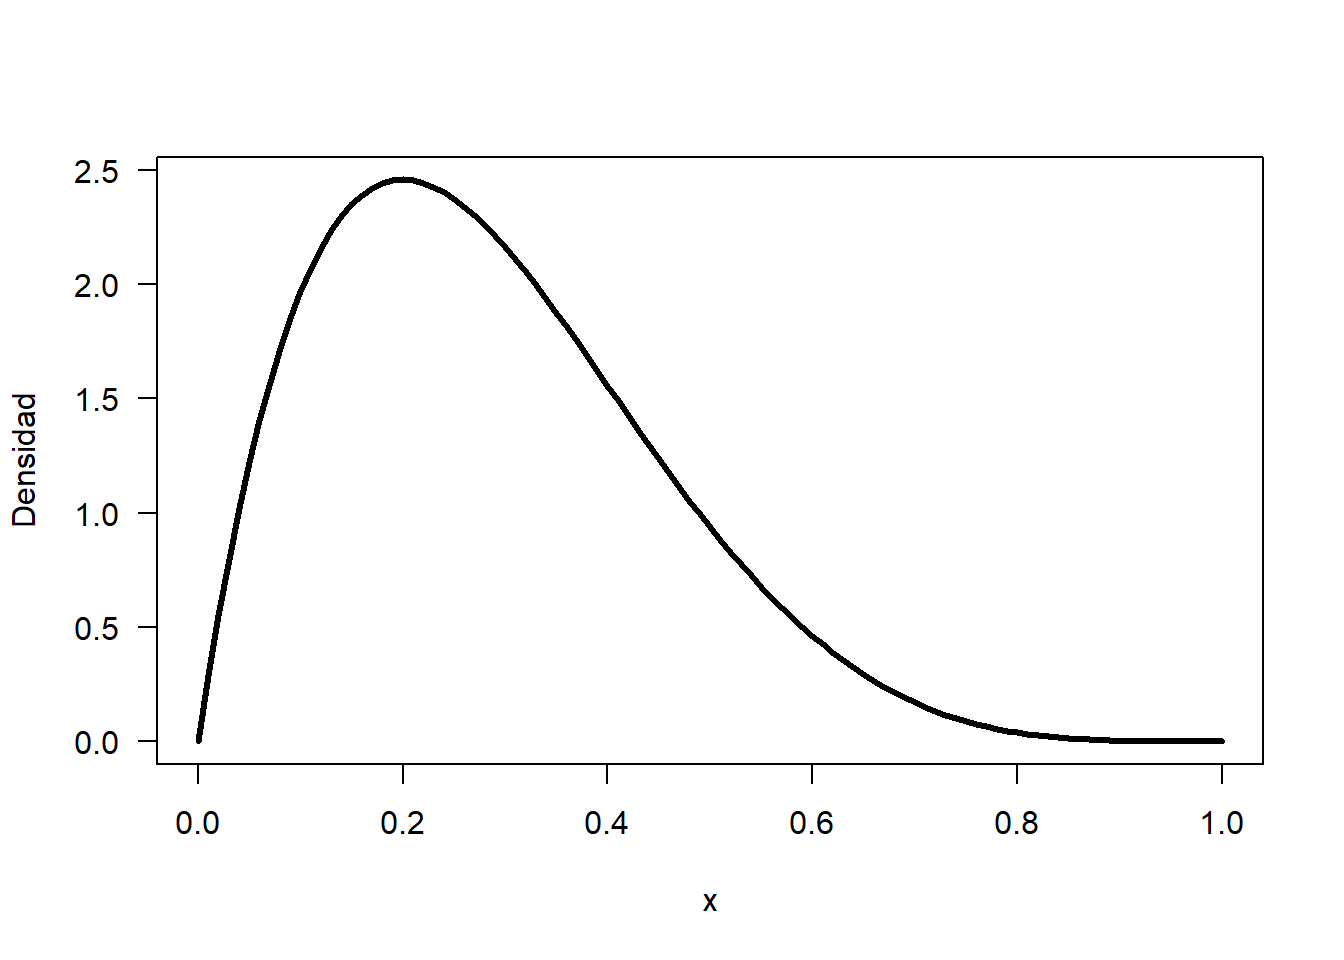
\includegraphics{disProbabilidad_files/figure-latex/unnamed-chunk-9-1.pdf}

\hypertarget{distribuciuxf3n-gamma}{%
\subsection{2. Distribución Gamma}\label{distribuciuxf3n-gamma}}

En este apartado, se explicarán las funciones existentes en R para
obtener resultados que se basen en la \textbf{distribución Gamma}.

\textbf{Para obtener valores que se basen en la distribución Gamma, R,
dispone de cuatro funciones:}

\begin{Shaded}
\begin{Highlighting}[]
\FunctionTok{dgamma}\NormalTok{(x, shape, rate, }\AttributeTok{scale =} \DecValTok{1}\SpecialCharTok{/}\NormalTok{rate, }\AttributeTok{log =}\NormalTok{ F)}\CommentTok{\#    Devuelve resultados de la función de densidad.}

\FunctionTok{pgamma}\NormalTok{(q, shape, rate, }\AttributeTok{scale =} \DecValTok{1}\SpecialCharTok{/}\NormalTok{rate, }\AttributeTok{lower.tail =}\NormalTok{ T, }\AttributeTok{log.p =}\NormalTok{ F)   }\CommentTok{\#Devuelve resultados de la función de distribución acumulada.}

\FunctionTok{qgamma}\NormalTok{(p, shape, rate, }\AttributeTok{scale =} \DecValTok{1}\SpecialCharTok{/}\NormalTok{rate, }\AttributeTok{lower.tail =}\NormalTok{ T, }\AttributeTok{log.p =}\NormalTok{ F)   }\CommentTok{\#Devuelve resultados de los cuantiles de la distribución Gamma.}

\FunctionTok{rgamma}\NormalTok{(n, shape, rate, }\AttributeTok{scale =} \DecValTok{1}\SpecialCharTok{/}\NormalTok{rate) }\CommentTok{\#    Devuelve un vector de valores de la distribución Gamma aleatorios.}
\end{Highlighting}
\end{Shaded}

\textbf{Los argumentos que podemos pasar a las funciones expuestas en la
anterior tabla, son:}

\begin{itemize}
\item
  \textbf{x, q:} Vector de cuantiles.
\item
  \textbf{p:} Vector de probabilidades.
\item
  \textbf{n:} Números de observaciones.
\item
  \textbf{rate:} Alternativa para especificar el valor de escala
  (Scale). Por defecto, su valor es igual a 1.
\item
  \textbf{shape}, \textbf{scale:} Parámetros de la Distribución Gamma.
  Shape = a y Scale = s = 1/rate. Debe ser estrictamente positivo el
  parámetro Scale.
\item
  \textbf{log}, \textbf{log.p:} Parámetro booleano, si es TRUE, las
  probabilidades p son devueltas como log (p).
\item
  \textbf{lower.tail:} Parámetro booleano, si es TRUE (por defecto), las
  probabilidades son \textbf{P{[}X ≤ x{]}}, de lo contrario,
  \textbf{P{[}X \textgreater{} x{]}}.
\end{itemize}

\hypertarget{ejercicio-de-aplicaciuxf3n-1}{%
\subsubsection{Ejercicio de
aplicación}\label{ejercicio-de-aplicaciuxf3n-1}}

\textbf{En cierta ciudad el consumo diario de energía eléctrica, en
millones de kilovatios por hora, puede considerarse como una variable
aleatoria con distribución Gamma de parámetros α = 3 y β = 0.5.}

La planta de energía de esta ciudad tiene una capacidad, suficiente
diaria de 10 millones de kW/hora, determinar la probabilidad de que este
abastecimientos sea: \textbf{Se consuman entre 3 y 8 millones de
kW/hora.}

\hypertarget{soluciuxf3n-2}{%
\paragraph{Solución}\label{soluciuxf3n-2}}

Nos piden, la probabilidad: \textbf{P(3 \textless X \textless8)},
empleamos para tal propósito, la función de distribución con el área de
cola hacia la izquierda y la alternativa para especificar el valor de
escala:

\begin{Shaded}
\begin{Highlighting}[]
\FunctionTok{pgamma}\NormalTok{(}\DecValTok{8}\NormalTok{, }\DecValTok{3}\NormalTok{, }\AttributeTok{rate =} \FloatTok{0.5}\NormalTok{, }\AttributeTok{lower.tail =}\NormalTok{ T) }\SpecialCharTok{{-}} \FunctionTok{pgamma}\NormalTok{(}\DecValTok{3}\NormalTok{, }\DecValTok{3}\NormalTok{, }\AttributeTok{rate =} \FloatTok{0.5}\NormalTok{, }\AttributeTok{lower.tail =}\NormalTok{ T)}
\end{Highlighting}
\end{Shaded}

\begin{verbatim}
## [1] 0.5707435
\end{verbatim}

\hypertarget{distribuciuxf3n-exponencial}{%
\subsection{3. Distribución
Exponencial}\label{distribuciuxf3n-exponencial}}

La distribución exponencial es una distribución de probabilidad continua
que se utiliza para modelar el tiempo o espacio entre eventos en un
proceso de Poisson.

La distribución exponencial es la distribución de probabilidad del
tiempo o espacio entre dos eventos en un proceso de Poisson, donde los
eventos ocurren de manera continua e independiente a una tasa constante
λ.

\textbf{Para obtener valores que se basen en la distribución
Exponencial, R, dispone de cuatro funciones:}

\begin{Shaded}
\begin{Highlighting}[]
\FunctionTok{dexp}\NormalTok{(x, }\AttributeTok{rate =} \DecValTok{1}\NormalTok{, }\AttributeTok{log =}\NormalTok{ F)  }\CommentTok{\#Devuelve resultados de la función de densidad.}
\FunctionTok{pexp}\NormalTok{(q, }\AttributeTok{rate =} \DecValTok{1}\NormalTok{, }\AttributeTok{lower.tail =}\NormalTok{ T, }\AttributeTok{log.p =}\NormalTok{ F)    }\CommentTok{\#Devuelve resultados de la función de distribución acumulada.}
\FunctionTok{qexp}\NormalTok{(p, }\AttributeTok{rate =} \DecValTok{1}\NormalTok{, }\AttributeTok{lower.tail =}\NormalTok{ T, }\AttributeTok{log.p =}\NormalTok{ F)    }\CommentTok{\#Devuelve resultados de los cuantiles de la distribución Exponencial.}
\FunctionTok{rexp}\NormalTok{(n, }\AttributeTok{rate =} \DecValTok{1}\NormalTok{)   }\CommentTok{\#Devuelve un vector de valores de la distribución Exponencial aleatorios}
\end{Highlighting}
\end{Shaded}

\textbf{Los argumentos que podemos pasar a las funciones expuestas en la
anterior tabla, son}

\begin{itemize}
\item
  \textbf{x}, \textbf{q}: Vector de cuantiles.
\item
  \textbf{p}: Vector de probabilidades.
\item
  \textbf{n}: Números de observaciones.
\item
  \textbf{rate}: Vector de tasas. Hay que tener en cuenta que:
  \textbf{rate = 1/β}
\item
  \textbf{log}, \textbf{log.p}: Parámetro booleano, si es TRUE, las
  probabilidades p son devueltas como \textbf{log(p)}.
\item
  \textbf{lower.tail}: Parámetro booleano, si es TRUE (por defecto), las
  probabilidades son \textbf{P{[}X ≤ x{]}}, de lo contrario,
  \textbf{P{[}X \textgreater{} x{]}}
\end{itemize}

\hypertarget{ejercicio-de-aplicaciuxf3n-2}{%
\subsubsection{Ejercicio de
aplicación}\label{ejercicio-de-aplicaciuxf3n-2}}

\textbf{Supongamos que la cantidad de tiempo que uno pasa en un banco se
distribuye exponencialmente con una media de 10 minutos,λ= 1/10 ¿Cuál es
la probabilidad de que un cliente pase más de 15 minutos en el banco si
aún está en el banco? después de 10 minutos?}

\hypertarget{soluciuxf3n-3}{%
\paragraph{Solución}\label{soluciuxf3n-3}}

\[P(X>15|X>10)=P(X>5)=e^{-1/2} = 0.606\]

\begin{Shaded}
\begin{Highlighting}[]
\FunctionTok{pexp}\NormalTok{(}\DecValTok{5}\NormalTok{,}\AttributeTok{rate=}\DecValTok{1}\SpecialCharTok{/}\DecValTok{10}\NormalTok{,}\AttributeTok{lower.tail =} \ConstantTok{FALSE}\NormalTok{) }\CommentTok{\# o 1{-} Pexp(5,rate=1/10,lower.tail = TRUE)}
\end{Highlighting}
\end{Shaded}

\begin{verbatim}
## [1] 0.6065307
\end{verbatim}

\hypertarget{distribuciuxf3n-normal}{%
\subsection{4. Distribución Normal}\label{distribuciuxf3n-normal}}

Entre las variables aleatorias continuas, la más importante es la
distribución normal o gaussiana. Esta variable fue introducida por Carl
Friedrich en el siglo XIX para estudiar las medidas de error.

Sea \textbf{X∼N(μ,σ)}, es decir, una variable aleatoria con distribución
normal de media μ y desviación típica σ: \frac{a}{b+c}

\textbf{La función de densidad, también conocida como campana de Gauss,
de x es:}
\[f(x)=\frac{1}{\sqrt{2πσ^{2}}} e^{(1/2)(   \frac{x-μ}{σ})^{2}}\]

\textbf{La función de distribución acumulada} \[F(x)=P(X≤x)\]

\textbf{La esperanza y la varianza es} \[E(X)=μ ; Var(X)=σ^{2}\]

\textbf{donde:}

\begin{itemize}
\item
  \textbf{μ} es la media de la distribución (también la mediana y el
  modo).
\item
  \textbf{σ} es la desviación estándar
\item
  \textbf{(σ\textgreater0)}.
\item
  \textbf{σ\^{}2} varianza
\end{itemize}

\textbf{Para obtener valores que se basen en la distribución Normal, R,
dispone de cuatro funciones:}

\begin{Shaded}
\begin{Highlighting}[]
\FunctionTok{dnorm}\NormalTok{(x, }\AttributeTok{mean =} \DecValTok{0}\NormalTok{, }\AttributeTok{sd =} \DecValTok{1}\NormalTok{, }\AttributeTok{log =}\NormalTok{ F)}\CommentTok{\#    Devuelve resultados de la función de densidad.}

\FunctionTok{pnorm}\NormalTok{(q, }\AttributeTok{mean =} \DecValTok{0}\NormalTok{, }\AttributeTok{sd =} \DecValTok{1}\NormalTok{, }\AttributeTok{lower.tail =}\NormalTok{ T, }\AttributeTok{log.p =}\NormalTok{ F)   }\CommentTok{\#Devuelve resultados de la función de distribución acumulada.}

\FunctionTok{qnorm}\NormalTok{(p, }\AttributeTok{mean =} \DecValTok{0}\NormalTok{, }\AttributeTok{sd =} \DecValTok{1}\NormalTok{, }\AttributeTok{lower.tail =}\NormalTok{ T, }\AttributeTok{log.p =}\NormalTok{ F)   }\CommentTok{\#Devuelve resultados de los cuantiles de la Normal.}

\FunctionTok{rnorm}\NormalTok{(n, }\AttributeTok{mean =} \DecValTok{0}\NormalTok{, }\AttributeTok{sd =} \DecValTok{1}\NormalTok{)}\CommentTok{\# Devuelve un vector de valores de la Normal aleatorios.}
\end{Highlighting}
\end{Shaded}

\textbf{Los argumentos que podemos pasar a las funciones expuestas en la
anterior tabla, son:}

\begin{itemize}
\item
  \textbf{x}, q: Vector de cuantiles.
\item
  \textbf{p}: Vector de probabilidades.
\item
  \textbf{n}: Números de observaciones.
\item
  \textbf{mean}: Vector de medias. Por defecto, su valor es \textbf{0}.
\item
  \textbf{sd}: Vector de desviación estándar. Por defecto, su valor es
  \textbf{1}.
\item
  \textbf{log}, *\textbf{log.p}: Parámetro booleano, si es TRUE, las
  probabilidades p son devueltas como \textbf{log(p)}.
\item
  \textbf{lower.tail}: Parámetro booleano, si es TRUE (por defecto), las
  probabilidades son \textbf{P{[}X ≤ x{]}}, de lo contrario,
  \textbf{P{[}X \textgreater{} x{]}}.
\end{itemize}

\hypertarget{ejercicio-1-de-aplicaciuxf3n}{%
\subsubsection{Ejercicio 1 de
aplicación}\label{ejercicio-1-de-aplicaciuxf3n}}

\textbf{En el siguiente ejemplo, observamos la gráfica de la función de
distribución acumulada para una variable aleatoria X que tiene
distribución normal con parámetros μ=2 y σ=1.1:}

\begin{Shaded}
\begin{Highlighting}[]
\CommentTok{\# Crear una sucesión de números entre {-}9 y 9, aumentando en 0.05.}
\NormalTok{x }\OtherTok{\textless{}{-}} \FunctionTok{seq}\NormalTok{(}\SpecialCharTok{{-}}\DecValTok{9}\NormalTok{, }\DecValTok{9}\NormalTok{, }\AttributeTok{by =} \FloatTok{0.05}\NormalTok{)}

\CommentTok{\# Suponiendo que los parámetros son: mu=2 y sigma=1.1.}
\NormalTok{y }\OtherTok{\textless{}{-}} \FunctionTok{pnorm}\NormalTok{(x, }\AttributeTok{mean =} \DecValTok{2}\NormalTok{, }\AttributeTok{sd =} \FloatTok{1.1}\NormalTok{)}

\CommentTok{\# Gráfica de la densidad normal}
\FunctionTok{plot}\NormalTok{(x,y)}
\end{Highlighting}
\end{Shaded}

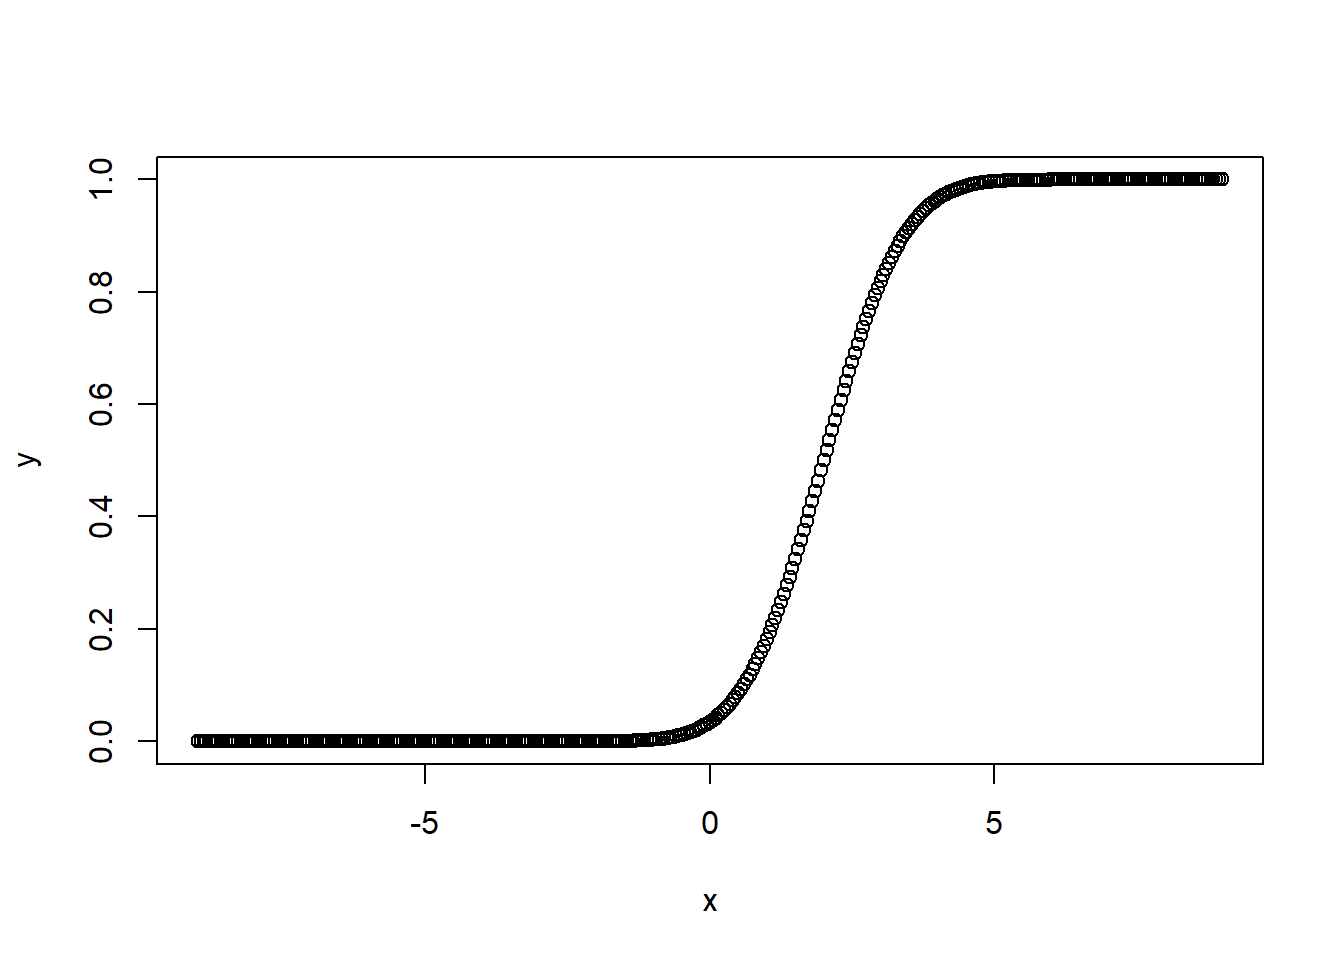
\includegraphics{disProbabilidad_files/figure-latex/unnamed-chunk-15-1.pdf}

\hypertarget{ejercicio-2-de-aplicaciuxf3n}{%
\subsubsection{Ejercicio 2 de
aplicación}\label{ejercicio-2-de-aplicaciuxf3n}}

\textbf{Si X es una variable normal con media μ=50 y varianza
σ\^{}2=100, calcule la probabilidad de que X se encuentre entre -60 y
60.}

\hypertarget{soluciuxf3n-4}{%
\paragraph{Solución}\label{soluciuxf3n-4}}

\textbf{La probabilidad de que X se encuentre entre -60 y 60 (ambos
inclusive) es:} \begin{eqnarray*}
    P(|X| \leq 60) &=& P(-60 \leq X  \leq 60)\; =\;  P(X\leq 60) \; - \; P(X\leq -60) \\
     &=&  P\Big(Z \leq \frac{60-50}{10}\Big) \; - \;  P\Big(Z \leq \frac{-60-50}{10}\Big)\\
     &=& P(Z \leq 1) - P(Z\leq -11) = 0.8413  - 0 \; =\; 0.8413
\end{eqnarray*}

\hypertarget{soluciuxf3n-en-r}{%
\paragraph{Solución en R}\label{soluciuxf3n-en-r}}

\begin{Shaded}
\begin{Highlighting}[]
\FunctionTok{pnorm}\NormalTok{(}\DecValTok{60}\NormalTok{,}\DecValTok{50}\NormalTok{,}\FunctionTok{sqrt}\NormalTok{(}\DecValTok{100}\NormalTok{))}\SpecialCharTok{{-}}\FunctionTok{pnorm}\NormalTok{(}\SpecialCharTok{{-}}\DecValTok{60}\NormalTok{,}\DecValTok{50}\NormalTok{,}\FunctionTok{sqrt}\NormalTok{(}\DecValTok{100}\NormalTok{))}
\end{Highlighting}
\end{Shaded}

\begin{verbatim}
## [1] 0.8413447
\end{verbatim}

\hypertarget{distribuciuxf3n-t-de-student}{%
\subsection{5. Distribución t de
Student}\label{distribuciuxf3n-t-de-student}}

la distribución \textbf{T de Student} es una distribución de
probabilidad que surge del problema de estimar la media de una población
normalmente distribuida cuando el tamaño de la muestra es pequeño y la
desviación estándar poblacional es desconocida

Existe la fórmula para calcular el valor de \textbf{t} en la
distribuciones \textbf{T Student..} Se usa la siguiente fórmula para
transformar distribuciones normales a \textbf{t}.

\[t=\frac{\bar{x}-u}{\frac{s}{\sqrt{n}}}\] \textbf{donde:}

\[\bar{x}\text{=media muestral}\]

\[μ \text{=media poblacional}\]

\[s\text{=desviación estándar de la muestra}\]

\[n\text{=número de elementos de la muestra}\]

\textbf{Para obtener valores que se basen en la distribución t-Student,
R, dispone de cuatro funciones:}

\begin{Shaded}
\begin{Highlighting}[]
\FunctionTok{dt}\NormalTok{(x, df, ncp, }\AttributeTok{log =}\NormalTok{ F)}\CommentTok{\#    Devuelve resultados de la función de densidad.}

\FunctionTok{pt}\NormalTok{(q, df, ncp, }\AttributeTok{lower.tail =}\NormalTok{ T, }\AttributeTok{log.p =}\NormalTok{ F)}\CommentTok{\#  Devuelve resultados de la función de distribución acumulada.}

\FunctionTok{qt}\NormalTok{(p, df, ncp, }\AttributeTok{lower.tail =}\NormalTok{ T, }\AttributeTok{log.p =}\NormalTok{ F)   }\CommentTok{\#Devuelve resultados de los cuantiles de la t{-}Student.}

\FunctionTok{rt}\NormalTok{(n, df, ncp)}\CommentTok{\# Devuelve un vector de valores de la t{-}Student aleatorios.}
\end{Highlighting}
\end{Shaded}

\textbf{Los argumentos que podemos pasar a las funciones expuestas en la
anterior tabla, son:}

\begin{itemize}
\item
  \textbf{x}, \textbf{q}: Vector de cuantiles.
\item
  \textbf{p}: Vector de probabilidades.
\item
  \textbf{n}: Números de observaciones.
\item
  \textbf{df}: Grados de libertad.
\item
  \textbf{ncp}: Parámetro que determina la centralidad de la gráfica
  t-Student. Si se omite, el estudio se realiza con la gráfica
  centralizada en 0.
\item
  \textbf{log}, \textbf{log.p}: Parámetro booleano, si es TRUE, las
  probabilidades p son devueltas como \textbf{log(p)}.
\item
  \textbf{lower.tail}: Parámetro booleano, si es TRUE (por defecto), las
  probabilidades son \textbf{P{[}X ≤ x{]}}, de lo contrario,
  \textbf{P{[}X \textgreater{} x{]}}
\end{itemize}

\hypertarget{ejercicio-de-aplicaciuxf3n-3}{%
\subsubsection{Ejercicio de
aplicación}\label{ejercicio-de-aplicaciuxf3n-3}}

\textbf{Un Gerente de mall desea estimar la cantidad media que gastan
los clientes que visitan el centro comercial. Una muestra de 20 clientes
revela las siguientes cantidades: 48.16, 42.22,46.82, 51.45, 23.78,
41.86, 54.86, 37.92, 52.64, 48.59, 50.82, 46.94, 61.83, 61.69, 49.17,
61.46, 51.35, 52.68, 58.84, 43.88}

datos:

\begin{Shaded}
\begin{Highlighting}[]
\NormalTok{dato }\OtherTok{\textless{}{-}} \FunctionTok{c}\NormalTok{(}\FloatTok{48.16}\NormalTok{, }\FloatTok{42.22}\NormalTok{, }\FloatTok{46.82}\NormalTok{, }\FloatTok{51.45}\NormalTok{, }\FloatTok{23.78}\NormalTok{, }\FloatTok{41.86}\NormalTok{, }\FloatTok{54.86}\NormalTok{, }\FloatTok{37.92}\NormalTok{, }\FloatTok{52.64}\NormalTok{, }\FloatTok{48.59}\NormalTok{, }\FloatTok{50.82}\NormalTok{, }\FloatTok{46.94}\NormalTok{, }\FloatTok{61.83}\NormalTok{, }\FloatTok{61.69}\NormalTok{, }\FloatTok{49.17}\NormalTok{, }\FloatTok{61.46}\NormalTok{, }\FloatTok{51.35}\NormalTok{, }\FloatTok{52.68}\NormalTok{, }\FloatTok{58.84}\NormalTok{, }\FloatTok{43.88}\NormalTok{)}
\NormalTok{media }\OtherTok{\textless{}{-}} \FunctionTok{round}\NormalTok{(}\FunctionTok{mean}\NormalTok{(dato),}\DecValTok{4}\NormalTok{)}
\NormalTok{desviacion }\OtherTok{\textless{}{-}} \FunctionTok{round}\NormalTok{(}\FunctionTok{sd}\NormalTok{(dato),)}
\NormalTok{n }\OtherTok{\textless{}{-}} \FunctionTok{length}\NormalTok{(dato)}
\NormalTok{confianza }\OtherTok{\textless{}{-}} \FloatTok{0.95}
\end{Highlighting}
\end{Shaded}

\textbf{Construir una tabla de datos}

\begin{Shaded}
\begin{Highlighting}[]
\NormalTok{tabla }\OtherTok{\textless{}{-}} \FunctionTok{data.frame}\NormalTok{(}\AttributeTok{variables =} \FunctionTok{c}\NormalTok{(}\StringTok{"n"}\NormalTok{, }\StringTok{"Grados libertad"}\NormalTok{, }\StringTok{"Media muestra"}\NormalTok{, }\StringTok{"Desv.Std muestra"}\NormalTok{, }\StringTok{"Media Pob."}\NormalTok{, }\StringTok{"Confianza"}\NormalTok{), }\AttributeTok{datos =} \FunctionTok{c}\NormalTok{(n, (n}\DecValTok{{-}1}\NormalTok{), media, desviacion, }\ConstantTok{NA}\NormalTok{, confianza)) }
\NormalTok{tabla}
\end{Highlighting}
\end{Shaded}

\begin{verbatim}
##          variables  datos
## 1                n 20.000
## 2  Grados libertad 19.000
## 3    Media muestra 49.348
## 4 Desv.Std muestra  9.000
## 5       Media Pob.     NA
## 6        Confianza  0.950
\end{verbatim}

\textbf{Valor de t real}

\begin{Shaded}
\begin{Highlighting}[]
\NormalTok{t }\OtherTok{\textless{}{-}} \FunctionTok{qt}\NormalTok{(}\AttributeTok{p =}\NormalTok{ (}\DecValTok{1} \SpecialCharTok{{-}}\NormalTok{ confianza) }\SpecialCharTok{/} \DecValTok{2}\NormalTok{, }\AttributeTok{df =}\NormalTok{ n}\DecValTok{{-}1}\NormalTok{) }\CommentTok{\# dos colas}
\NormalTok{t }\OtherTok{\textless{}{-}} \FunctionTok{abs}\NormalTok{(t)}
\NormalTok{t}
\end{Highlighting}
\end{Shaded}

\begin{verbatim}
## [1] 2.093024
\end{verbatim}

\end{document}
